\documentclass[a4paper]{article}

\usepackage{color}
\usepackage{url}
\usepackage[T2A]{fontenc} % enable Cyrillic fonts
\usepackage[utf8]{inputenc} % make weird characters work
\usepackage{graphicx}

\usepackage[english,serbian]{babel}
%\usepackage[english,serbianc]{babel} %ukljuciti babel sa ovim opcijama, umesto gornjim, ukoliko se koristi cirilica

\usepackage[unicode]{hyperref}
\hypersetup{colorlinks,citecolor=green,filecolor=green,linkcolor=blue,urlcolor=blue}

%\newtheorem{primer}{Пример}[section] %ćirilični primer
\newtheorem{primer}{Primer}[section]

\begin{document}

\title{Pametni (elektricni) automobili u 2022. godini\vspace{3ex}\\ \small{Seminarski rad u okviru kursa\\Tehničko i naučno pisanje\\ Matematički fakultet}}

\author{\\\\\\Nera Zejak\\Eleonora Jovanović Kisseleva\\Nemanja Potić\\Kristijan Petronijević \\ \\nerazejak1130@gmail.com\\eleonorajovanovic1@gmail.com\\x.nemanjapotic.x@gmail.com\\ petronijevick3@gmail.com\\}
\date{1.~novembar 2022.}
\maketitle

\abstract{
 U narednom tekstu ćemo se ukratko upoznati sa \textbf{Pametnim (električnim) automobilima.} Počev od toga šta su pametni automobili, objasnićemo šta su osnove bioinformatike, kao i mnoge zanimljive činjenice ove jedinstvene interdisciplinarne oblasti. Razgovaramo o glavnim principima koji podupiru bioinformatičke analize, razmatramo tipove bioloških informacija i baza podataka koje se obično koriste.}


\tableofcontents

\newpage

\section{Uvod}
   Električni automobil (primer jednog na slici \ref{fig:IMG_Tesla}) je automobil koji se pokreće elektromotorom, koristeći \textbf{električnu energiju} pohranjenu u akumulatoru, ili drugim uređajima za pohranu energije. Električni automobili su bili popularni krajem 19. i početkom 20. veka. 
        


\begin{figure}[h]
        \centering
        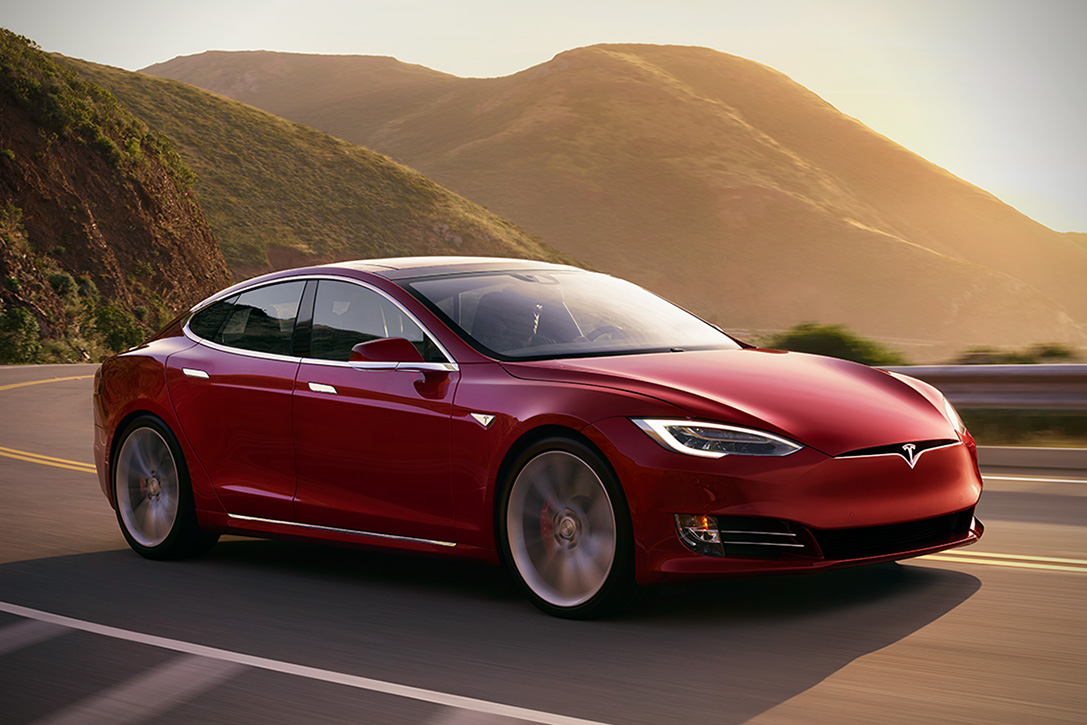
\includegraphics[width=\linewidth]{tesla.jpeg}
        \caption{Tesla model S}
        \label{fig:IMG_Tesla}
        \end{figure}
        Unapređenja motora sa unutarnjim sagorevanjem i masovna proizvodnja jeftinijeg vozila na benzin doveli do smanjenja korišćenja vozila na električni pogon.
         Energetske krize 1970-ih i 80-ih dovele su do kratkotrajnog zanimanja za \textbf{električne automobile}, te se sredinom 2000. obnovio interes za proizvodnjom električnih automobila, uglavnom zbog zabrinutosti oko ubrzanog povećanja cene nafte i potrebe za smanjenjem emisije gasova staklene bašte.
         
\label{sec:uvod}






\section{Popularnost električnih automobila}
\label{slike_i_tabele}

Najnoviji izveštaj "Bloomberg New Energy" pokazuje da će do 2040. godine 58\% globalne prodaje dolaziti od električnih automobila. Istovremeno oni će činiti nešto manje od 33\% ukupnih automobila na putu.




\begin{primer} U narednoj tabeli \ref{tab:tabela1} videćemo zemlje kod kojih je porcenat novih automobila sa električnim pogonom najveći.


\begin{table}[h!]
\begin{center}
\caption{Procenat kupljenih automobila sa električnim pogonom za 2022 godinu.}
\begin{tabular}{|c|c|c|} \hline
Norveška& Island& Švedska\\ \hline
58\% &18\%&11\%\\ \hline
\end{tabular}
\label{tab:tabela1}
\end{center}
\end{table}

\end{primer}





\section{Istorija}
\label{sec:naslov1}


Električna vozila su u upotrebi već skoro 2 veka i ona se smatraju sledećim korakom ka održivijem i više ekološki prihvatljivijom urbanom transportu. Njihova popularnost i upotreba raste od početka 21. veka, kada je interesovanje za njih poraslo zbog uticaja na životnu sredinu od strane emisija koja prave vozila koja rade na fosilnim gorivima. Potražnja za električnim automobilima će nastaviti da raste zbog toga što potrošači uvek traže način da smanje troškove, a cene električnih automobila vremenom opadaju i njihovom upotrebom nema potrebe za dodatnim troškovima na goriva.


\subsection{Rana istorija}
\label{subsec:podnaslov1}

Praktična električna vozila su se prvi put pojavila 90-ih godina 19. veka i ona su držala rekord u brzini vozila do oko 1900-te godine. Električna energija je bila među poželjnijim metodoma automobilskog pogona jer je pružala nivo lakoće rada i udobnosti koju automobili na benzin tog vremena nisu mogli da pruže.

Električna vozila su se koristila kao privatna motorna vozila do 20. veka, kada je zbog niskih maksimalnih brzina i visokih cena u poređenju sa vozilima sa SUS motorima\footnote{Motori sa unutrašnjim sagorevanjem tj. SUS motori su toplotni motori kod kojih produkti sagorevanja, svojim direktnim dejstvom vrše mehanički rad.} došlo do svetskog pada njihove upotrebe kao privatnih motornih vozila. Odlučujući momenat u ovom preokretu je bilo uvođenje elektropokretača tj. anlasera\footnote{Elektropokretač (anlaser) je elektromotor namenjen za pokretanje motora sa unutrašnjim sagorevanjem.} 1912. godine. koji je zamenio druge metode pokretanja SUS motora. Jedna od zamenjenih metoda je bila pokretanje kurblom\footnote{Kurbla je valjkasta šipka napravljena od gvožđa.} koju je bilo potrebno okretati naglo i snažno sve dok se SUS motor ne bi upalio.

Električna vozila su se idalje koristila za javni prevoz i kao utovarna i teretna oprema, ali se tek u na početku 21. veka interesovanje za njihovu upotrebu kao privatna vozila ponovo povećalo.


\subsection{Moderni električni automobili}
\label{subsec:podnaslov2}


Na početku 21. veka je došlo do porasta zabrinutosti zbog štete po životnu sredinu urzokovanu emisijama koje prave vozila koja rade na fosilnim gorivima. CARB\footnote{CARB (California Air Reasources Board) je agencija za čist vazduh u vladi Kalifornije.} se već u ranim 90-im godinama 20. veka borila za upotrebu vozila koja ispuštaju manje štetnih gasova, sa krajnjim ciljem da se koriste vozila koja ih uopšte neće ispuštati, kao što su, na primer, električna.

Dobar deo zasluge za povećanje interesovanja za električne automobile je bilo prouzrokovano od strane \textbf{dva događaja}.

\begin{itemize}
\item  \textbf{Prvi događaj} je bio pojava Toyota Prius-a, modela koji je počeo da se porizvodi u Japanu 1997. godine. On je postao prvo svetsko hibridno električno vozilo\footnote{Hibridno električno vozilo je tip hibridnog vozila koje kombinuje konvencialni sistem SUS motora zajedno sa električnim pogonskim sistemom.} koje je imalo masivnu proizvodnju. U 2000. godini je počeo da se prodaje širom sveta i vrlo brzo je postao popularan među poznatim ličnostima, što je znatno podiglo profil modela vozila. Za njegovu proizvodnju Toyota\footnote{Toyota Motor Corporation, poznatija kao Toyota, je japanski proizvođač automobila, baziran u gradu Tojota.} je koristila nikl-metal hidridnu bateriju\footnote{Nikl-metal hidridna baterija (Ni-MH) je vrsta punjive baterije koje se obično koriste kao zamena za nepunjive alkalne baterije sličnog oblika.}, tehnologiju podržanu od strane odeljenja za istraživanje energije. Prius je postao najprodavaniji hibrid širom sveta u poslednjoj deceniji zahvaljujući porastu cena benzina i zabrinutosti zbog zagađenja ugljenikom.
\item \textbf{Drugi događaj} je bila vest u 2006. godini o tome da će kompanija Tesla Motors\footnote{Tesla Motors je bivši naziv automobilske i elektroenergetske kompanije Tesla.} početi da proizvodi model luksuznih električnih sportskih automobila koji će moći da idu više od 320 km sa jednim punjenjem. Ona je već 2004. godine krenula  sa razvojem datog automobila, a 2008. godine ga je i dostavila klijentima. Ime modela je Tesla Rodster i on je prvi potpuno električni automobil legalan na autoputu i prvi proizvodni potpuno električni automobil koji putuje više od 320 km.
\end{itemize} 


Kompanija Mitsubishi Motors je 2009. godine u Japanu počela da prodaje Mitsubishi i-MIEV, prvi električni automobil legalan na autoputu koji se serijski proizvodio. Ovaj model automobila je takođe prvi koji je prodat u više od 10,000 primeraka.

U 2008. godini su počele promene u proizvodnji električnih automobila zbog napredaka baterija, cilja da se smanje emisije gasova staklene bašte i da se poboljša kvalitet vazduha.

Tesla Model 3 je u martu 2020. godine prestigao Nissan Leaf\footnote{Nissan Leaf je električno vozilo proizvedeno od strane Nissan-a, japanskog multinacionalnog proizvođača automobila.} i postao najprodavaniji električni automobil svih vremena, sa više od 500,000 prodatih primeraka. U junu 2021. godine je dostigao 1.000.000 globalno prodatih primeraka.


\subsection{Budućnost električnih automobila}
\label{subsec:podnaslov3}


Ne možemo tačno utvrditi šta sledi električhnim automobilima u budućnosti, ali trenutno oni imaju ogroman potencijal da učine tu budućnost ekološki održivijom. U transportnom sektori oni bi mogli da potpuno zamene fosilna goriva, da povećaju energetsku efikasnost i da smanje zagađenje.

U pitanje se dovode i potencijalni problemi koje bi korišćenje samo električnih vozila dovelo. Jedan od problema je pitanje dugoročne održivosti električnih vozila zbog rizika koji predstavlja nabavka kritičnih materijalnih resursa koji se koriste u baterijama električnih automobila. Eksploatacija nekih od ovih resursa je povezana sa značajnim uticajima na životnu sredinu, kao i sa društvenim i etičkim pitanjima. 

\section{Princip rada električnih automobila\vspace{2ex}}

Električni automobili se oslanjaju na električne baterije, umesto na benzin ili dizel, te na taj način obezbeđuju energiju za rad. Električna energija se crpi iz velike punjive baterije i šalje se kroz niz komponenti pre nego što dođe do elektromotora. Pre nego što se energija dopremi motoru, jednosmerna struja koju daje baterija se pretvori u naizmeničnu struju.

\section{Princip rada električnih automobila\vspace{2ex}}

Električni automobili se oslanjaju na električne baterije, umesto na benzin ili dizel, te na taj način obezbeđuju energiju za rad. Električna energija se crpi iz velike punjive baterije i šalje se kroz niz komponenti pre nego što dođe do elektromotora. Pre nego što se energija dopremi motoru, jednosmerna struja koju daje baterija se pretvori u naizmeničnu struju.
Potrebno je da se ispravna količina snage prenese na motor, a to omogućavaju \textbf{potenciometri} (vrsta promenljivog otpora koji može da odoleva struji koja teće kroz strujno kolo).U električnim vozilima su kablom povezani sa papučicom gasa. Kada vozač pritisne papučicu za gas, što veći pritisak vrši, to manji otpor imaju potenciometri. Električna vozila obično imaju dva potenciometra, a snaga se dostavlja motoru samo ako su oba postavljena u istom položaju. Ovo omogućava da ukoliko dođe do kvara jednog od potenciometara, a papučica gasa je puštena, auto će se postepeno zaustavljati umesto da se izgubi kontrola pri visokim brzinama. Jedna od ključnih komponenti je i \textbf{regulator} koji kontroliše koliko električne energije stiže do motora električnog vozila. Regulator dobija informaciju koliko je pritiska upotrebljeno na papučicu gasa primanjem podataka sa dva potenciometra. Sa tim informacijama reguliše koliko snage se šalje u motor. U regulatoru se jednismerna struja iz baterije pretvara u naizmeničnu struju koja pokreće motor koji dalje pokreće točkove i omogućava kretanje vozila. 

\section{Modeli automobila koji su obeležili 2022. godinu\vspace{2ex}}
\label{sec:MODELI AUTOMOBILA KOJI SU OBELEŽILI 2022. GODINU}

   Prošla godina je protekla kao i 2020. u borbi sa pandemijom, ali je svaka fabrika prolazila i kroz svoje probleme koji su se odnosili na nestašicu čipova. Drugu polovinu 2021. godine obeležio je i pad proizvodnje i prodaje automobila. Izostale su takođe i brojne premijere novih modela koje su odložene za ovu godinu. SUV vozila\footnote{SUV (Sport utility vehicle) je terenski automobil, vrsta automobila velike nosivosti, vučne snage i putničkog kapaciteta.} ostaju i dalje popularna i najtraženija, a očigledno je da ćemo viđati sve više električnih automobila sa sve većim dometom.\\\\

    Ono što je novina u autoindustriji je da će još jedan sistem postati deo obavezne opreme automobila. Sa tom uredbom se krenulo od jula ove godine. Evropska komisija usvojila je nacrt uredbe kojom se definiše obavezna ugradnja uređaja za “inteligentno prilagođavanje brzine”\footnote{Intelligent speed assistance (ISA) je svaki sistem koji obezbeđuje to da brzina vozila ne prelazi bezbednu, ili zakaonom propisanu brzinu.} na svim novim vozilima i to od 6. jula 2022. godine. Sve nas naravno interesuje i kakve će boje biti aktuelne. Proteklih godina dominirale su siva i crna, a zatim je iznenada bela postala omiljena kod kupaca. Naročito je tražena kad su u pitanju SUV vozila. Što se tiče boja mnogi su dali titulu  trendsetera Hyundai modelima\footnote{Hyndai Motor Company (Hyndai Motors) je južnokorejski multinacionalni proizvođač automobila.}.
    \\\\
    Ovo su neki od modela sa kojima ćemo se upoznati, a koje su predstavili poznate ili neke novije auto kuće:\\
    \begin{itemize}
     \item ŠKODA ENYAQ IV 
     \item RENAULT AUSTRAL   
     \item MERCEDES-BENZ VISION EQXX 
     \item EVOLUTE I-PRO 
     \item DRAKO DRAGON\\ 
    \end{itemize}
    
\maketitle{\textbf{ŠKODA ENYAQ IV}}
\\

    Škoda je 31. januara 2022. godine predstavila svoj novi ENYAQ COUPÉ iV koji možete videti na slici \ref{fig:IMG_Enyaq}. To je električni top model češkog proizvođača automobila. S koeficijentom otpora od 0,234, ENYAQ COUPÉ iV je predvodnik u svojoj klasi, što ga čini posebno efikasnim u vožnji. \\
    Poput modela ENYAQ iV, novi ŠKODA ENYAQ COUPÉ iV takođe se temelji na modularnoj platformi (MEB) Volkswagen grupe. S koeficijentom otpora od cd 0,234, elegantni coupé postaće predvodnika+ u svom segmentu i poboljšaće već odličnu vrednost modela ŠKODA ENYAQ iV, delom zahvaljujući novom obliku karoserije\footnote{Karoserija je gornji deo motornog vozila koji se pričvršćuje na osnovni donji deo vozila koji se naziva šasija ili ram.}.\\ 

\begin{figure}[h]
        \centering
        \includegraphics[width=\linewidth]{ENYAQ COUPÉ iV.png}
        \caption{ENYAQ COUPÉ iV}
        \label{fig:IMG_Enyaq}
\end{figure}

\newpage

\maketitle{\textbf{RENAULT AUSTRAL}}
\\

    Renault za ovu godinu je imao cilj da osvoji C-segment\footnote{C-segment tj. niža srednja klasa je treća kategorija evropskih segmenata za putnička vozila.} sa novim SUV-om pod nazivom Austral (prikazan na slici \ref{fig:IMG_Austral}). Zadržane su temeljne karakteristike koje SUV-ove čine privlačnima. Ipak, novi dizajnerski pristup i novi oblici predstavljaju pomak od tradicionalnih i statičnih vodoravnih linija, postavljenih u ravni sa tlom. Austral se ističe oštrim i dinamičnim linijama, naglašenim bočnim linijama, ali i novim oblikom svetala. Dva velika zadnja svetla u obliku slova C stapaju se sa središnjim logotipom.\\  

\begin{figure}[h]
        \centering
        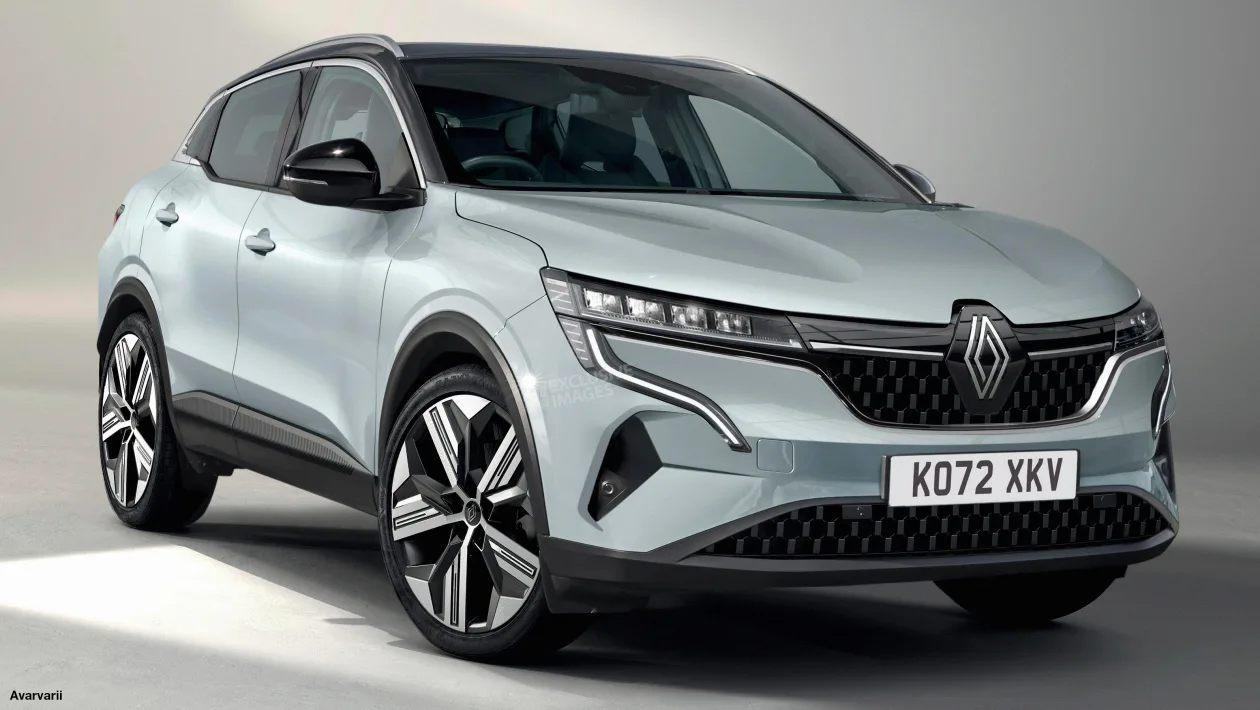
\includegraphics[width=\linewidth]{Austral.jpg}
        \caption{RENAULT AUSTRAL}
        \label{fig:IMG_Austral}
        \end{figure}

\newpage

\maketitle{\textbf{MERCEDES-BENZ VISION EQXX}}
\\

    Ovaj model (prikazan na slici \ref{fig:IMG_Mercedes}) se smatra za  “najefikasniji ikada izrađen Mercedes”. To nije prvi konstruisan novi masovno proizvedeni električni Mercedes EQS ili pak EQE, već potpuno nov automobil. On je dakle osmišljen na novim osnovama od samih početaka razvoja. Novitet predstavlja neku vrstu manifesta za diviziju Mercedes-EQ nemačke grupacije Daimler koja se bavi elektromobilima i kao takav daje uvid u smer razvoja kompanijskih baterijskih modela.\\ 
 

\begin{figure}[h]
        \centering
        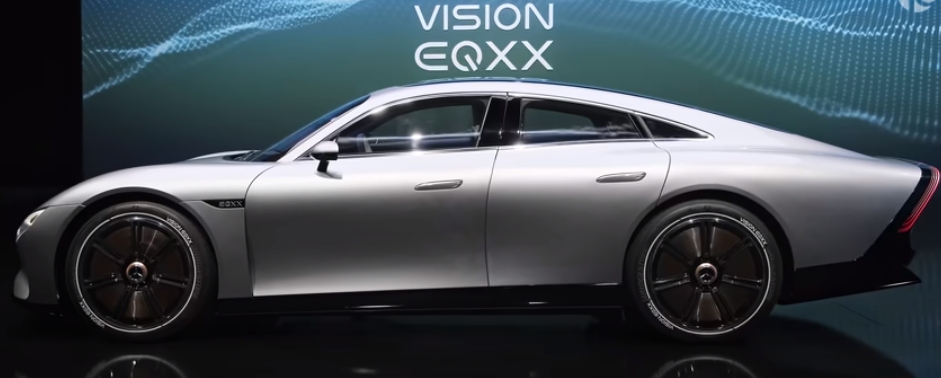
\includegraphics[width=\linewidth]{Vision.png}
        \caption{MERCEDES-BENZ VISION EQXX}
        \label{fig:IMG_Mercedes}
        \end{figure}


\maketitle{\textbf{EVOLUTE I-PRO}}
\\

    U Rusiji je počela prodaja prvog električnog automobila proizvedenog u toj zemlji, saopštio je proizvođač MotorInvest, javlja Anadolija. Lansiranje prvih ruskih proizvedenih električnih vozila pod brendom Evolute održano je krajem septembra u zapadnoj regiji Lipeck. I-Pro limuzina je bila prvi model koji iz proizvodne trake pušten u prodaju.\\
    Evolute i-Pro limuzina (prikazana na slici \ref{fig:IMG_EVOLUTE}) je opremljena vučnom baterijom kapaciteta 53 kilovata (kW) i ostvaruje domet do 420 kilometara. Električni motor ima 150 konjskih snaga.
    Početna cena automobila je tri miliona rubalja (oko 50.000 dolara). Prodajna mreža MotorInvesta pokriva devet regiona Rusije: Moskvu, Sankt Peterburg, Nižnji Novgorod, Kazanj, Voronjež, Lipeck, Krasnodar, Rostov na Donu i Soči.\\
    Do kraja godine MotorInvest planira da u prodaju pustiti i modele iJoy crossover te iVan minivan. Modeli će koštati 3,49 miliona rubalja, a 2023. će se pojaviti i-Jet cross-coupe. Ukupno, do kraja godine, kompanija namjerava proizvesti 2.000 električnih vozila.\\ 
    
    \newpage
    
    \begin{figure}[h]
        \centering
        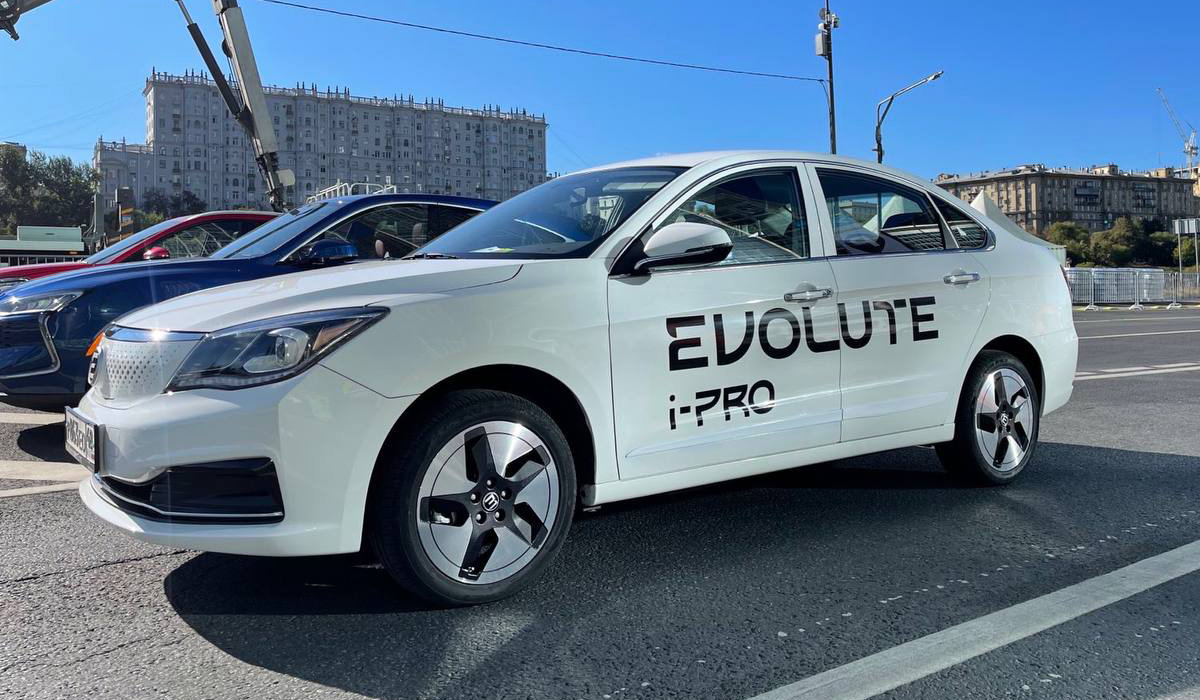
\includegraphics[width=\linewidth]{evoluteipro.jpg}
        \caption{EVOLUTE I-PRO}
        \label{fig:IMG_EVOLUTE}
        \end{figure}


\maketitle{\textbf{DRAKO DRAGON}}
\\

    Kompanija Drako Motors je nedavno održala premijeru svog novog modela, a to je električni hyper-SUV Dragon (prikazan na slici \ref{fig:img_DRAKO}). 
    Dragon SUV sa gull-wing vratima\footnote{Gull-wing vrata (falcon-wing vrata) su vrata automobila koja su šarkama zakačena na krov, a ne sa strane vozila.} je baziran na kompanijinoj arhitekturi Drako DriveOS i ima Drako DriveOS Quad Motor pogonski sistem. U pitanju je postavka sa četiri električna motora i ukupno 2000KS. Prema najavama, to će omogućiti ubrzanje od 0 do 60 milja na sat (96 km/h) za 1,9 sekundi.
    Najveća brzina ovog 2254 kg teškog vozila iznosi više od 200 milja na sat (322 km/h), dok četvrt milje (402 metra) može da se pređe za 9,0 sekundi. Što se dometa tiče, sa jednim punjenjem Dragon može da pređe do 676 km. Dragon je dugačak 5054 mm, postavljen je na točkove od 23 inča, a u kabini nudi mesta za pet putnika.
    Drako Motors već prima rezervacije za prvu seriju od 99 vozila. Cene startuju od 290.000 dolara, ali isporuke neće početi pre 2026. godine. U planu je da se kasnije proizvodi 5.000 primeraka godišnje.
 
\begin{figure}[h]
        \centering
        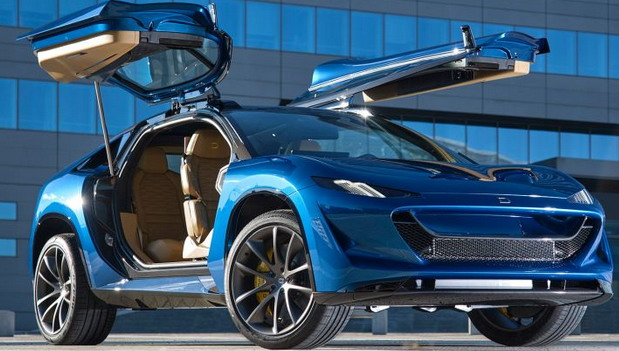
\includegraphics[width=\linewidth]{DRAKO.jpg}
        \caption{DRAKO DRAGON}
        \label{fig:img_DRAKO}
        \end{figure}


\newpage

\section{Zaključak}
\label{sec:zakljucak}

Elektricni automobili koji su ujedno i pametni imaju svoje prednosti i mane. Motori na elektro pogon ne zagadjuju okolinu ali tu se javlja problem punjena baterija koji nije bas najbrzi proces.


\addcontentsline{toc}{section}{Literatura}
\appendix

\iffalse
\bibliography{seminarski} 
\bibliographystyle{plain}
\fi

\begin{thebibliography}{9}

\bibitem{laski2009software} J. Laski and W. Stanley. \emph{Software Verification and Analysis}. Springer- Verlag, London, 2009.

\bibitem{gcc} Free Software Foundation. GNU gcc, 2013. on-line at: http://gcc. gnu.org/.

\bibitem{haltingproblem} A. M. Turing. \emph{On Computable Numbers, with an application to the Entscheidungsproblem}. Proceedings of the London Mathematical Society, 2(42):230–265, 1936.


\end{thebibliography}





\end{document}
